\documentclass[journal,twoside,web]{ieeecolor}
\usepackage{generic}

% TODO: subfigures
% TODO: update subfigure references
% TODO: change graph roc-auc to percentage
% TODO: check
%The maximum depth a graphic can be
%is 8.5 inches (216 millimeters/54 picas). When choosing the
%depth of a graphic, please allow space for a caption
% TODO: check png dpi 300dpi.
% TODO: check data->plural
% TODO: check issue->problem
% TODO: remove duplicate references
% TODO: remove unused references
% TODO: Other than books, capitalize only the first word in a paper
% title, except for proper nouns and element symbols.
% TODO: punctuate equations
% TODO: IEEE-style graphs
% TODO: use algorithmic
% TODO: eqref etc to ensure Fig. 1 format
% TODO: Remove textcite
% TODO: abbreviate journals/conferences in bib
% TODO: only capitalize first word in references
% TODO: replace latent by core if not talking about forward/backward model
% TODO: LLM spellcheck
% TODO: vim spellcheck
% TODO: compile figures independently to pdf
%Figures (line artwork or photographs) should be named
%starting with the first 5 letters of the author’s last name. The
%next characters in the filename should be the number that
%represents the sequential location of this image in your article.
%For example, in author “Anderson’s” paper, the first three
%figures would be named ander1.tif, ander2.tif, and ander3.ps.

\usepackage{bttda-paper}

\addbibresource{references.bib}
\addbibresource{moabb_datasets.bib}

\begin{document}

\title{Block-Term Tensor Discriminant Analysis for Brain-Computer Interfacing}

\author{%
	Arne Van Den Kerchove,
	Hakim Si-Mohammed,
	Fran\c{c}ois Cabestaing,
	Marc M. Van Hulle, \IEEEmembership{Fellow, IEEE}
	\thanks{%
		Submitted for review on \today.
		This work was supported in part by the special research fund of the KU Leuven
		(GPUDL/20/031) and the University of Lille under the Global PhD Scholarship Program,
		the European Union’s Horizon Europe Marie Sklodowska-Curie Action program
		(grant agreement No. 101118964), the European Union’s Horizon 2020 research and
		innovation program (grant agreement No. 857375), the special research fund of
		the KU Leuven (C24/18/098), the Belgian Fund for Scientific Research – Flanders
		(G0A4118N, G0A4321N, G0C1522N), and the Hercules Foundation (AKUL 043).
		The authors acknowledge the support of the RITMEA project co-financed by the
		European Union with the European Regional Development Fund, the French state,
		and the Hauts-de-France Region Council.
	}
	\thanks{%
		Arne Van Den Kerchove is with the Department of Neuroscience, KU Leuven,
		BE-3000 Leuven, Belgium
		He is affiliated with the CRIStAL joint research group at University of Lille,
		CNRS, and Centrale Lille, France(e-mail: arne.vandenkerchove.com).
	}
	\thanks{%
		Hakim Si-Mohammed (e-mail: hakim.si-mohammed@univ-lille.fr) and Fran\c{c}ois
		Cabestaing (e-mail: francois.cabestaing@univ-lille.fr) are with the CRIStAL
		joint research group  (UMR 9189) at University of Lille, CNRS, and Centrale
		Lille, FR-59655 Villeneuve d'Ascq, France.
	}
	\thanks{%
		Marc M. Van Hulle is with the Department of Neuroscience, KU Leuven.
		He is a senior member of the Leuven Brain Institute and the Leuven.AI institute
		for Artificial Intelligence (email: marc.vanhulle@kuleuven.be).
	}
}

\maketitle

\begin{abstract}
	\input{abstract.txt}
\end{abstract}

\begin{IEEEkeywords}
	tensor discriminant analysis,
	brain-computer interface,
	block-term decomposition,
	multilinear decoding,
	event-related potentials,
	motor imagery

\end{IEEEkeywords}

\section{Introduction}

\Acp{bci} have the potential to bypass
defective neural pathways by providing an alternative communication channel
between the brain and an external device, with applications in
neuroprosthetics, assistive technologies and rehabilitation~\cite{Wolpaw2020}.
\Acp{bci} record and process neural signals, with \ac{eeg} the most popular
recording method in the field.
A \ac{bci} usually identifies specific, task-related activity in
the recorded signal, coupling it to output or actions.
This methodology often gives rise to classification problems~\cite{Lotte2018}.
Some well-known examples include the P300 speller~\cite{Krusienski2006}, where
momentary visual stimuli evoke characteristic \acp{erp} modulated by attention,
and \ac{mi}~\cite{Aggarwal2019}, where different (imagined) limb movements evoke
\acp{ersd} with different spatial patterns.
As a consequence, decoding (\ac{erp} vs.\ non-attended \ac{erp}, left
vs.\ right limb \ac{mi}, \ldots) involves classifier training with labeled
\ac{eeg} data (calibration) and applying it to unseen \ac{eeg} data
(operation).

%User experience is enhanced by minimizing calibration session duration session
%duration.
%This results in small, subject- and session-specific training datasets
%exposing decoders to overfitting in the presence of high-dimensional data.
%Dimensionality reduction techniques mitigate this risk by extracting extracts a
%lower-dimensional set features relevant to the classification problem at hand.

\subsection{Tensors \& tensor methods}

Due to their multichannel time series nature, \ac{eeg} and other functional
neuroimaging data naturally exist as multiway data, capturing
information in both the spatial and the temporal domain.
Preprocessing transformations can further expand this data into additional
analytic domains.
Common examples include time-frequency transformation, time-binning, or
integrating information across multiple subjects or conditions.
These high-dimensional datasets which are usually flattened
into a set of sample vectors, stripping the original data of its structure.
\emph{Tensors}, multiway arrays with each domain
corresponding to a tensor \emph{mode}, are a more suitable and structured
representation exploiting the intrinsic multiway structure of neural
data~\cite{Erol2022}.
This in turn paves the way to tensor methods counteracting some drawbacks of
high dimensionality.
Tensor methods are machine learning or dimensionality reduction techniques treating
each tensor mode separately, reducing a given problem into partial per-mode problems.

Tensor methods often decompose a tensor into a lower dimensional
core tensor and set of factor matrices, adhering to either the Tucker
or PARAFAC structure.
A Tucker decomposition reduces an input tensor of order $K$ with dimensions
$(D_1,D_2,\ldots,D_K)$ to a dense core with dimensions $(R_1,R_2,\ldots,R_K)$,
with $R_k \leq D_k$ for $k=1, 2, \ldots K$ using per-mode factor matrices.
The \ac{hosvd}~\cite{DeLathauwer2000,SoleCasals2018} performs unsupervised
Tucker decomposition and approximation.
Alternatively, \ac{parafac} methods decompose a tensor in a sum of rank-1
tensors, each the product of a scalar and per-mode factor vectors.
This is equivalent to the Tucker structure with all core elements off the hyperdiagonal
set to 0, as shown in \cref{fig:bttda/sparse}.
Canonical Polyadic Decomposition is an unsupervised \ac{parafac} method~\cite{Hitchcock1927,Nazarpour2006}.
These decompositions can extract features vectors from input data using the
flattened core tensors.
These can subsequently be classified to predict class labels, most
commonly using \ac{lda} or a \ac{svm}.
\begin{figure*}[t]
	\centering%
	\hfill%
	\footnotesize
\begin{tikzpicture}[x=\textwidth/14.2, y=-\textwidth/14.2, scale=0.75]
	\TensorThree{data}{}{}{}{2}{2}{2}
	\begin{scope}[shift={((5.5,0)}]
		\TensorThree{core}{}{}{}{1}{1}{1}
		\begin{scope}[shift={(-0.0707, -0.0707)}]
			\MatrixSkewed{fac. 1}{}{}{1}{1}
		\end{scope}
		\begin{scope}[shift={(-0.1,0)}]
			\MatrixLeft{fac. 2}{}{}{1}{1}
		\end{scope}
		\begin{scope}[shift={(0,1.1)}]
			\MatrixBelow{fac. 3}{}{}{1}{1}
		\end{scope}
	\end{scope}
	\draw[->] (2.5,1, -1) -- (3.75,1,-1);
\end{tikzpicture}
%
	\hfill\vrule\hfill%
	\footnotesize
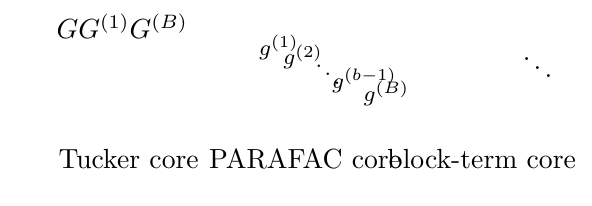
\begin{tikzpicture}[x=\textwidth/14.2, y=-\textwidth/14.2, scale=0.75]
	%\useasboundingbox (0,-1) rectangle (13,3.5);
	\TensorThree{$\ten{G}$}{}{}{}{2}{2}{2}
	\node[anchor=north, align=center] at (1,2) {Tucker core};

	{\footnotesize
	\begin{scope}[shift={(3.5,0)}]
		\TensorThree{}{}{}{}{2}{2}{2}
		\node at (.33,.33,-.33) {$g^{(1)}$};
		\node at (.66,.66,-.66) {$g^{(2)}$};
		\node at (1,1,-1) {$\ddots$};
		\node at (1.5, 1.5, -1.5) {$g^{(b-1)}$};
		\node at (1.8, 1.9, -1.8) {$g^{(B)}$};
	\end{scope}
	}
	\node[anchor=north, align=center] at (4.5,2) {PARAFAC core};

	\begin{scope}[shift={(7,0)}]
		\TensorThree{}{}{}{}{2}{2}{2}
		\TensorThree{$\ten{G}^{(1)}$}{}{}{}{.5}{.5}{.5}
		\node at (.75,.75,-.75) {$\ddots$};
		\begin{scope}[shift={(1,1,-1)}]
			\TensorThree{$\ten{G}^{(B)}$}{}{}{}{1}{1}{1}
		\end{scope}
	\end{scope}
	\node[anchor=north, align=center] at (8,2) {block-term core};
\end{tikzpicture}
%
	\hfill%
	\caption{%
		A tensor decomposition finds core tensor and factor matrices
		from input tensor.
		This core tensor can have several structures.
		In the Tucker structure, the core is a dense tensor $\ten{G}$.
		The \ac{parafac} structure expresses the core as a sum of $B$ rank-1 terms, each
		with a scalar core $g^{(b)}$.
		The block-term structure expresses the core as a sum of $B$ smaller,
		Tucker-structured blocks $\ten{G}^{(b)}$.
		Both the \ac{parafac} and block-term structures are more sparse than the full
		Tucker structure, yet the block-term structure is more flexible as it
		allows blocks of variable tensor dimensionality instead of fixed rank-1 terms.
	}\label{fig:bttda/sparse}%
\end{figure*}

Nevertheless, Tucker or \ac{parafac} structures might not efficiently represent
all relevant neural information in a compressed format.
%Performance of Tucker or \ac{parafac} methods are
%heavily dependent on prior choice of the hyperparameters determining dimension
%or the number of rank-1 terms.
The block-term tensor structure is a generalization of both the Tucker and
\ac{parafac} structures, representing a tensor as a sum of Tucker structured terms.
The \ac{btd}~\cite{DeLathauwer2008,DeLathauwer2008a,DeLathauwer2008b,Rontogiannis2021}
performs this decomposition in an unsupervised way.
If the number of terms is equal to 1, it is equivalent to the Tucker structure;
if the dimensions of each term are equal to 1, it is equivalent to the \ac{parafac}
structure.
The block-term structure (\cref{fig:bttda/sparse}, right) is more flexible than
either Tucker or \ac{parafac} structures and strikes a better
balance between extracting maximal relevant and minimal
irrelevant features.
However, this comes with a cost of more hyperparameters, as now
both the number of block terms and the dimensions of each term must be specified.

\subsection{Supervised tensor decompositions for \ac{bci}}

The Tucker, \ac{parafac} and block-term decompositions are generally not unique.
Hence, other optimization criteria than the unsupervised methods above can be applied.
Given low signal-to-noise ratio and specific, task-related output in \ac{bci}
decoding, supervised machine learning and feature extraction is
favored over unsupervised techniques~\cite{Lotte2018}.
Dimensionality reduction for classification ideally optimizes
class discriminability of the extracted features.
In this philosophy, \ac{hoda}~\cite{Yan2005,Phan2010,Froelich2018} performs Tucker-structured decomposition optimizing
for Fisher-sense class separability, analogous to Linear Discriminant Analysis.
Variants of \ac{hoda} have been applied to \ac{bci} problems such as \ac{erp}~\cite{Onishi2012,Higashi2016} and \ac{mi}~\cite{Liu2015,Cai2021} decoding, with positive
results~\cite{Lotte2018}.
Further work proposes optimized objective functions or
regularizations~\cite{JamshidiIdaji2017,Jorajuria2022,Aghili2023}.
\Ac{parafac}-structured discriminant tensor decomposition has equally been
applied~\cite{Froelich2018}, but it is not trivial whether Tucker or \ac{parafac}
most suited for neural data in \ac{bci} decoding.

Recent work adopts more performant flexible structures.
\Ac{hopls}~\cite{Zhao2012,Camarrone2018} and \ac{bttr}~\cite{Faes2022,Faes2022a}
with parameter-free model selection achieve promising results for \ac{bci}
regression tasks.
\Ac{bttr} has also been adapted into classification variant
\ac{bttc}~\cite{Camarrone2021} but this methodology leaves room for improvement:
instead of optimizing directly for class separability, \ac{bttc} regresses
to dummy binary variable.
Thus, \ac{bttc} cannot be extended to multi-class settings.
Furthermore, core structures are still relatively constrained.
\textcite{Huang2020} propose a supervised approach for finding multiple discriminant
multilinear spectral filter terms applied to to \ac{mi}, yet their
decomposition is also restricted to terms with dimension $(R_1,R_2,1)$ with mode 3
the frequency domain.
A full block-term tensor structure could provide a more flexible approach if
directly optimized for discriminability.

\subsection{Contribution: A block-term structured model for classification}

With a proper choice of reduced dimension and number of terms, a
supervised block-term decomposition might be more suited to represent
complex discriminant neural data in a sparse way and yielding a regularizing effect.
Feature extraction with multiple, low-dimensional parsimonious discriminant block
terms might improve performance over a single \ac{hoda} block requiring
high dimensions to capture discriminant information, which in turn extracts many
irrelevant features.
From a complementary viewpoint:
if \ac{hoda} with well-chosen reduced dimensions extracts some discriminant
features, it is likely that not all useful information is extracted due to
the Tucker structure constraints.
Could \ac{hoda} therefore not sequentially be applied to extract more discriminant
Tucker structured terms -- potentially with lower dimension -- as long as decoding
performance improves?

We implement a novel supervised feature
extraction method titled \ac{bttda}, a generalization of \ac{hoda}.
\Ac{bttda} extracts discriminant features while adhering to a
flexible and efficient block-term tensor structure.
This work features the following contributions:
1) We develop a forward model for \ac{hoda} to reconstruct a given input tensor
from the extracted features.
2) This allows us to introduce \ac{bttda}\footnote{The source code of the
	methods introduced in this work is available at
	\url{https://github.com/arnevdk/bttda}.} as a state-of-the-art \ac{bci}
feature extraction method based on the block-term tensor structure.
3) We evaluate \ac{bci} decoders based on \ac{bttda} on decoding benchmarks for
both \ac{erp} and \ac{mi} \ac{bci} paradigms and compare performance to
state-of-the-art decoders.

\section{Methods}

\subsection{Notation}
Bold letters $\mat{U}$ indicate matrices,  bold underlined letters $\ten{X}$
indicate tensors. Uppercase letters $K$ represent fixed scalars and lowercase letters $k$.
variable scalars.
The $n^\text{th}$ sample of a tensor dataset with $N$ samples is written as
$\ten{X}(n)$, the dataset itself as ${\{\ten{X}(n)\}}_n^N$.
A tensor $\smash{\ten{X}\in \mathbb{R}^{D_1\times D_2 \times \cdots \times D_K}}$ can be
unfolded in mode $k$ to a matrix
$\smash{\mat{X}_k\in\mathbb{R}^{(D_k\times\prod_{j\neq k}^K D_j)}}$, by concatenating
all mode $j\neq k$ fibers.
The tensor-matrix product of tensor $\ten{X}$ with matrix $\mat{U}$ along a
given mode $k$ is written as $\ten{X}\mpr{\mat{U}}{k}$.
For ease of notation, let
$\ten{X}\mmpr{\mat{U}} =
	\ten{X}\mpr{\mat{U}}{1}\mpr{\mat{U}}{2}\cdots\mpr{\mat{U}}{K}$.
When skipping one of the modes $k$, this becomes
$\ten{X}\mmprs{\mat{U}}{k} =
	\ten{X}\mpr{\mat{U}}{1}\mpr{\mat{U}}{2}\cdots\mpr{\mat{U}}{k-1}\mpr{\mat{U}}{k+1}\ldots\mpr{\mat{U}}{K}$.
$\mat{A}\otimes\mat{B}$ indicates the Kronecker product of matrices $\mat{A}$
and $\mat{B}$.

\subsection{\Acl{hoda}}
\Acf{hoda}~\cite{Phan2010} is a supervised dimensionality reduction tensor
method for classification feature extraction.
For a set of $N$ tensors of order $K$
$\left\{\ten{X}(n)\in\mathbb{R}^{D_1\times D_2 \times \cdots \times
		D_K}\right\}_n^N$, HODA finds projection matrices $\mat{U_k}$ for each mode $k$
which project a given $\ten{X}$ to a latent tensor
$\ten{G}\in\mathbb{R}^{R_1\times R_2\times\cdots\times R_K}$, usually with lower
dimensions $(R_1\leq D_1,R_2\leq D_2,\ldots,R_K\leq D_K)$ using
tensor-matrix mode products:
\begin{equation}
	\ten{G}  = \ten{X}\mmpr{\mat{U}}
	\label{eq:HODA-backward}
\end{equation}
as visualized in \cref{fig:hoda/bw}.
\begin{figure*}
	\hfill%
	\begin{subfigure}{0.35\linewidth}%
		\centering%
		\footnotesize
\begin{tikzpicture}[y=-1cm, scale=0.75]
	\begin{scope}[shift={(0,0.5)}]
		\TensorThree{$\ten{G}$}{$R_1$}{$R_2$}{$R_3$}{1}{1}{1}
		\node at (2,0.5) {$=$};
	\end{scope}
	\begin{scope}[shift={(4.2,0)}]
		\TensorThree{$\ten{X}$}{}{}{}{2}{2}{2}
		\begin{scope}[shift={(-0.0707, -0.0707)}]
			\MatrixSkewed{$\mat{U}_1$}{$D_1$}{$R_1$}{1}{2}
		\end{scope}
		\begin{scope}[shift={(-0.1,0)}]
			\MatrixLeft{$\mat{U}_2$}{$D_2$}{$R_2$}{1}{2}
		\end{scope}
		\begin{scope}[shift={(0,2.1)}]
			\MatrixBelow{$\mat{U}_3$}{$D_3$}{$R_3$}{2}{1}
		\end{scope}
	\end{scope}
\end{tikzpicture}
%
		\caption{\Acs{hoda} backward model.}\label{fig:hoda/bw}%
	\end{subfigure}%
	%\hfill\vrule\hfill%
	\hfill%
	\begin{subfigure}{0.5\linewidth}%
		\centering%
		\footnotesize
\begin{tikzpicture}[y=-1cm, scale=0.75]
	\TensorThree{$\ten{X}$}{$D_1$}{$D_2$}{$D_3$}{2}{2}{2}
	\node at (3.25,.5){$=$};

	\begin{scope}[shift={(6.45,0)}]
		\begin{scope}[shift={(-0.0707, -0.0707)}]
			\MatrixSkewed{$\mat{A}_1$}{$R_1$}{$D_1$}{2}{1}
		\end{scope}
		\begin{scope}[shift={(-0.1,0)}]
			\MatrixLeft{$\mat{A}_2$}{$R_2$}{$D_2$}{2}{1}
		\end{scope}
		\begin{scope}[shift={(0,1.1)}]
			\MatrixBelow{$\mat{A}_3$}{$R_3$}{$D_3$}{1}{2}
		\end{scope}
		\TensorThree{$\ten{G}$}{}{}{}{1}{1}{1}

		\node at (1.75,.5){$+$};

		\begin{scope}[shift={(2.25,0)}]
			\TensorThree{$\ten{E}$}{}{}{}{2}{2}{2}
		\end{scope}


	\end{scope}



\end{tikzpicture}
%
		\caption{\ac{hoda} Forward model.}\label{fig:hoda/fw}
	\end{subfigure}%
	\hfill%
	\caption{%
		\Acf{hoda}.
		\subref{fig:hoda/bw} The multilinear projection applied
		to a third-order tensor sample $\ten{X}$ with dimensions $(D_1,D_2, D_3)$.
		\Ac{hoda} finds projection matrices $\mat{U}_k$ such that maximal
		discriminability between classes is achieved in the projected latent tensors
		$\ten{G}$ with reduced dimension $(R_1,R_2,R_3)$.
		\subref{fig:hoda/fw} By calculating activation patterns $\mat{A}_k$, the original tensor
		$\ten{X}$ can approximately be reconstructed from projected latent tensor $\ten{G}$.
		The reconstruction is accurate up to an error term $\ten{E}$.
	}
\end{figure*}
Since \ac{hoda} extracts latent features $\ten{G}$ from the observed data
$\ten{X}$ based a task-related criterion, it can be referred to as a
\emph{backward model}.

Analogous to \ac{hosvd}, \ac{hoda} decomposes $\ten{X}$ in a dense latent
tensor $\ten{G}$ and set of orthogonal projection matrices (weights) $\mat{U}_k$ to ensure uniqueness.
While \ac{hosvd} minimizes the reconstruction error,
\ac{hoda} optimizes  class discriminability of the reduced tensors
$\ten{G}(n)$ belonging to classes with labels $c_n$.
Discriminability is defined in the Fisher sense, maximizing Fisher ratio $\phi$
\begin{equation}
	\phi\left(\left\{\mat{U}\right\}\right) = \frac{\sum_c^CN_c\left\|\bar{\ten{G}}(c)-\bar{\bar{\ten{G}}}\right\|_F^2}
	{\sum_n^N\left\|\ten{G}(n)-\bar{\ten{G}}(c_n)\right\|_F^2}
	\label{eq:fisher}
\end{equation}
for $C$ classes with each $N_c$ samples.
$\bar{\ten{G}}(c)$ is the mean of
latent tensors of class $c$, and $\bar{\bar{\ten{G}}}$ the mean of
these class mean latent tensors.
If dimensions $(R_1,R_2, \ldots,R_k)$ are set a priori, the objective is now
to find the discriminant projection matrices:
\begin{equation}
	\left\{\mat{U}^*\right\} =  \argmax_{\{\mat{U}\}}\phi\left(\left\{\mat{U}\right\}\right)
\end{equation}
solved by \cref{alg:HODA}.

First, $\mat{U}_k$ are initialized to orthogonal matrices, e.g.,\ as random
orthonormal matrices, a per-mode \ac{svd}, or the partial \ac{hosvd} of the dataset.
The algorithm then iteratively loops over the modes fixing all
projections but $\mat{U}_k$ corresponding to mode $k$ and extracting
a partial latent tensor:
\begin{equation}
	\ten{G}_{-k}=\ten{X}\mmprs{\mat{U}}{k}
\end{equation}
Analogous to Linear Discriminant Analysis, new projection matrix $\mat{V}_k$
is calculated from the partial within-class scatter matrix:
\begin{equation}
	\mat{S}_{-k,\text{w}} = \sum_n^N\tilde{\mat{G}}_{-k,k}(n)\cdot\tilde{\mat{G}}_{-k,k}^\intercal(n)
\end{equation}
with $\tilde{\ten{G}}_{-k}(n) = \ten{G}_{-k}(n) - \bar{\ten{G}}_{-k}(c_n)$,
and the partial between-class scatter matrix:
\begin{equation}
	\mat{S}_{-k,\text{b}} =
	\sum_c^CN_c\tilde{\bar{\mat{G}}}_{-k,k}(c)\cdot\tilde{\bar{\mat{G}}}_{-k,k}^\intercal(c)
\end{equation}
with $\tilde{\bar{\ten{G}}}_{-k}(c) = \bar{\ten{G}}_{-k}(c) - \bar{\bar{\ten{G}}}_{-k}$,
by solving the eigenvalue problem:
\begin{equation}
	\mat{S}_{-k,\text{b}}-\varphi_k\mat{S}_{-k,\text{w}} =
	\mat{V}_k\mat{\Lambda}\mat{V}_k^\intercal
\end{equation}
for the first $R_k$ leading eigenvectors,
with $\varphi_k=\tr\left(\mat{U}_k^\intercal\mat{S}_{-k,\text{b}}\mat{U}_k\right)/\tr\left(\mat{U}_k^\intercal\mat{S}_{-k,\text{w}}\mat{U}_k\right)$
and $\mat{U}_k$ from the previous iteration.
Finally, the orthogonal transformation invariant projections $\mat{U}_k$
are obtained using per-mode total scatter matrices~\cite{Wang2007}:
\begin{equation}
	\mat{S}_{k,\text{t}} = \sum_n^N\mat{X}_k(n)\cdot\mat{X}_k^\intercal(n)
\end{equation}
and finding the $R_k$ leading eigenvectors of:
\begin{equation}
	\mat{V}_k\mat{V}_k^\intercal\mat{S}_{k,\text{t}}\mat{V}_k\mat{V}_k^\intercal
	= \mat{U}_k\mat{\Lambda}\mat{U}_k^\intercal
\end{equation}
The iterative process halts when each $\mat{U}_k$ update drops below a
predetermined threshold $\epsilon$ or after predetermined $I_\text{max}$ iterations.
\begin{algorithm}
	\caption[The \acs{hoda} backward solution.]{The \acs{hoda} backward solution.}
	\label{alg:HODA}
	\input{algorithms/alg_hoda_bw.tex}
\end{algorithm}

For classification with \ac{hoda}, projections are learned from a training
dataset with known class labels during calibration.
These projections extract core tensors from the training tensors, which
are then reshaped (\emph{vectorized}) into feature vectors
$\mat{g} =  \vect(\ten{G})$ together with the class labels to train a decision classifier.
In operation, learned projections extract core tensors from unseen test data
which are also vectorized and passed to the trained decision
classifier.

To avoid overfitting and improve performance in low sample size settings,
\ac{hoda} was regularized at each iteration by shrinking the partial
within-class scatter matrices~\cite{Phan2010} with a shrinkage factor
$\alpha_k$, such that the eigenvalue problems become
\begin{equation}
	\mat{S}_b^{(-k)} -
	\varphi\left[\left(1-\alpha_k\right)\mat{S}_{-k,\text{w}}+\alpha_k\mat{I}\right] =
	\mat{V}_k\mat{\Lambda}\mat{V}_k^\intercal
\end{equation}
As in Linear Discriminant Analysis, $\alpha_k$~\cite{Jorajuria2022}
estimates can be data-driven, e.g, using the Ledoit-Wolf procedure~\cite{Ledoit2003}.

\subsection{A forward model for \acs{hoda}}

As a prerequisite to the proposed \ac{bttda} model, we design a method to
reconstruct the original data tensor $\ten{X}$ from $\ten{G}$ after
dimensionality reduction as accurately as possible.
This requires a \emph{forward} model, a generative model expressing observed data in
terms of given latent features.
Forward models are useful for interpretability and data compression,
but \ac{bttda} relies on reconstruction with minimal error.
\Cref{eq:HODA-forward} gives a straightforward and computationally efficient
\ac{hoda} forward model candidate, visualized in \cref{fig:hoda/fw}:
\begin{equation}
	\ten{X} = \ten{G}\mmpr{\mat{A}^\intercal} + \ten{E} =
	\hat{\ten{X}} + \ten{E}
	\label{eq:HODA-forward}
\end{equation}
with \emph{activation patterns} $\mat{A}_k \in \mathbb{R}^{D_k\times R_k}$,
reconstructed tensor $\hat{\ten{X}}$, and error term $\ten{E}$.

A proper forward model minimizes the reconstruction error norm
$\left\|\ten{E}\right\|_F$.
%In other words, variation captured in the latent tensor is maximally captured
%by the reconstruction term $\hat{\ten{X}}= \ten{G}\mmpr{\mat{A}^\intercal}$
%and not by the error term $\ten{E}$~\cite{Haufe2014}.
%Hence, we minimize the expected value of the cross-covariance between
%the noise term and extracted latent tensors, or, equivalently
%\begin{equation}
%	\left\{\mat{A}^*\right\}
%	= \argmin_{\{\mat{A}\}}\text{E}\left[
%		\text{vec}\left(\ten{E}(n)\right)\text{vec}\left(\ten{G}(n)\right)
%		\right]_n
%\end{equation}
%or, equivalently~\cite{Parra2005,Haufe2014},
Hence, \cref{alg:HODA-fw} finds activation patterns~\cite{Parra2005, Haufe2014}
as
\begin{align}
	\left\{\mat{A}^*\right\}
	 & = \argmin_{\{\mat{A}\}}\sum_n^N\left[\ten{X}(n) -
	\hat{\ten{X}}(n)\right]^2                                                              \\
	 & = \argmin_{\{\mat{A}\}}\sum_n^N\left[\ten{X}(n) - \ten{G}(n)\mmpr{\mat{A}}\right]^2
\end{align}
This least-squares tensor approximation problem can be solved using the
Alternating Least Squares algorithm~\cite{Bentbib2022}, iteratively fixing all
but one of the activation patterns such that:
\begin{equation}
	\mat{A}_k = \argmin_{\mat{A}_k}
	\sum_n^N\left[\mat{X}_k(n) -
		\mat{A}_k\left(\ten{G}(n)\mmprs{\mat{A}}{k}\right)_k\right]^2
\end{equation}
which can be solved directly by ordinary least squares.
Activation patterns are initialized to the weights $\{\mat{U}\}$ of the
backward model.
Similar to fitting the backward model, the iterative process for the forward
model halts after a iterations $I_\text{max}$ iterations or when the update of each
$\mat{A}_k$ drops below $\epsilon$.
\begin{algorithm}
	\caption[A \acs{hoda} forward solution.]{The \acs{hoda} forward solution.}
	\label{alg:HODA-fw}
	\input{algorithms/alg_hoda_fw.tex}
\end{algorithm}

\subsection{\Acl{bttda}}
The \ac{hoda} forward model allows constructing the proposed discriminant
block-term tensor model.
If core tensors $\ten{G}$ after \ac{hoda} backward projection do not
perfectly separate classes, error term $\ten{E}$ in
\cref{eq:HODA-forward} contains further discriminative information
which can be exploited to improve classifier performance.
Extra features are extracted from $\ten{E} = \ten{X} -
	\hat{\ten{X}}$ by further projecting it onto another core tensor
$\ten{G}^{(2)}$, assuming $\ten{G}$ as $\ten{G}^{(1)}$.
Hence, we thus extend \ac{hoda} to \acf{bttda}, extracting multiple discriminative
latent blocks such that its forward model adheres to block-term tensor
structure:
\begin{equation}
	\ten{X} = \sum_b^B\ten{G}^{(b)}\mmpr{\mat{A}^{(b)}} + \ten{E}
	\label{eq:BTTDA-forward}
\end{equation}
for $B$ extracted latent tensors $\ten{G}^{(b)}$ and residual error term
$\ten{E}$ as illustrated by~\cref{fig:BTTDA}.
\begin{figure*}[t]
	\centering
	\input{figures/bttda_fw.tikz.tex}
	\caption[A forward model for \acs{bttda}.]{A forward model for \acf{bttda}.
		\Ac{bttda} can extract more features
		than \ac{hoda} by iteratively finding latent tensors $\ten{G}^{(b)}$ in using
		deflation.
		The \ac{hoda} backward projection is first applied. Next, the
		input data is reconstructed via the HODA forward model and the
		difference between the two is found.
		Finally, this process is repeated with this difference as input data, until a
		desired number of blocks $B$ has been found.}
	\label{fig:BTTDA}
\end{figure*}
The block-term structure of this model implies a generalization of both
the Tucker-structured \ac{hoda} and PARAFAC-structured discriminant feature
extraction.
If $B$ in \cref{eq:BTTDA-forward} is set to one, \ac{bttda} is equivalent to
\ac{hoda}; if at each term $b$ the dimensions of the core tensor are
$(R_1^{(b)}=R_2^{(b)}=\ldots=R_K^{(b)}=1)$, a \ac{parafac} structure is assumed
resulting in \ac{parafacda}.

In addition to this forward specification of \ac{bttda}, a backward procedure
is required to extract latent tensors $\ten{G}^{(b)}$ given $\ten{X}$ for
feature extraction.
This is achieved through a deflation scheme summarized in \cref{alg:BTTDA}.
\begin{algorithm}
	\caption{\Ac{bttda} feature extraction.}
	\label{alg:BTTDA}
	\begin{algorithmic}[1]
	\Require $\{\ten{X}(n)\}_n^N, \{c_n\}_n^N, \{(R_1^{(b)},R_2^{(b)},\ldots,R_K^{(b)})\}_b^B$
	\State $\ten{E}(n)\gets\ten{X}(n)\ \forall n$
	\For{$b=1,2,\ldots,B$}
	\State $\{\mat{U}^{(b)}\}\gets$ \parbox[t]{5cm}{\textsc{hoda} on $\{\ten{E}(n)\}_n^N$ and
	$\{c_n\}_n^N$ with rank $(R_1^{(b)},R_2^{(b)},\ldots,R_K^{(b)})$}
	\State $\ten{G}^{(b)}(n)\gets\ten{E}(n)\mmpri{\mat{U}^{(b)}}\
		\forall n$
	\State $\{\mat{A}^{(b)}\}\gets$ \parbox[t]{5cm}{Forward \textsc{hoda} on
		$\{\ten{G}^{(b)}(n)\}_n^N$ and $\ten{E}$}
	\State
	$\hat{\ten{E}}(n)\gets\ten{G}^{(b)}(n)\mmpri{\mat{A}^{\intercal(b)}}\
		\forall n$
	\State
	$\ten{E}(n)\gets \ten{E}(n) - \hat{\ten{E}}(n) \forall n$

	\EndFor
\end{algorithmic}

\end{algorithm}
The latent tensor corresponding to each block $b$ is extracted using the
\ac{hoda} backward projection from the residual error term of the previous
block $\ten{E}^{(b-1)}$ as in \cref{eq:HODA-backward}:
\begin{equation}
	\ten{G}^{(b)} = \ten{E}^{(b-1)}\mmpr{\mat{U}^{(b)}}
\end{equation}
This residual error term is the difference between the previous error and its
reconstruction after backward and forward \ac{hoda} projection:
\begin{align}
	\ten{E}^{(b)} = \ten{E}^{(b-1)} - \hat{\ten{E}}^{(b-1)}
	= \ten{E}^{(b-1)} - \ten{G}^{(b)}\mmpr{\mat{A}^{\intercal(b)}}
\end{align}
with $\ten{E}^{(0)}=\ten{X}$.
Resulting latent tensors can be vectorized and concatenated
\begin{equation}
	\mat{g}
	=\left[\vect\left(\ten{G}^{(1)}\right)\
		\vect\left(\ten{G}^{(2)}\right)\
		\cdots\
		\vect\left(\ten{G}^{(B)}\right)\right]
\end{equation}
for classification similar to \ac{hoda}.


\subsection{Model and feature selection}
Similar to unsupervised \ac{btd}, \ac{bttda} performance is sensitive to the
number of blocks $B$ and their corresponding dimensions
$\{(R_1^{(b)}, R_2^{(b)}, \ldots,	R_K^{(b)})\}_b^B$.
If these are not known a priori from data insights, model selection is required.
Although computationally expensive, hyperparameters can be set through
cross-validated tuning.
To reduce the search space, we introduce hyperparameter $\smash{\theta \in [0,1]}$
controlling the dimensions of all blocks.
$\theta$ controls the sparsity of the \ac{bttda} solution, with $\theta=0$
corresponding to the \ac{parafacda} model with blocks with dimensions
$(1,1,\ldots,1)$, and $\theta=1$ corresponding to blocks of full rank $(D_1, D_2,\ldots,D_K)$.
For $0 < \theta < 1$, the dimensions of block $b$ are be determined as in
\textcite{Phan2010}:
$R_k$ are chosen as the number of components needed to explain a
proportion $\theta$ of the mode variability the input data.
For each block in \ac{bttda}, this is determined by eigenvalues of the per-mode
total scatter matrix of tensor $\ten{E}^{(b-1)}$ as
\begin{equation}
	\mat{S}_{k,\text{t}}^{(b)} = \sum_n^N\mat{E}_k^{(b-1)}(n)\cdot\mat{E}_k^{(b-1)\intercal}(n)
	= \mat{W}_k^{(b)}\mat{\Lambda}_k^{(b)}\mat{W}_k^{(b)\intercal}
\end{equation}
such that
\begin{equation}
	R_k^{(b)} = \argmin_{R\in 1,\ldots,D_k}\frac{\sum_r^R\lambda_{k,r}^{(b)}}{\sum_r^{D_k}\lambda_{k,r}^{(b)}} > \theta
\end{equation}

\Ac{hoda}, and by extension \ac{bttda}, can extract a substantial amount
of redundant features.
These should be dropped before proceeding to classification~\cite{Phan2010}.
Particularly in \ac{bttda}, redundant features can accumulate over the number of
blocks, hampering performance.
Furthermore, discriminant features across blocks can be heavily correlated since
each block independently optimizes the discriminability criterion.
To mitigate this, extracted features are first decorrelated and scaled using
whitening \ac{pca}.
Relevant components are selected by univariate Fisher score
$\phi(i)$ calculated as:
\begin{equation}
	\phi(i) = \frac
	{\sum_c^C N_c \left[\bar{g}_i(c)-\bar{\bar{g}}_i\right]^2}
	{\sum_n^N \left[g_i(n)-\bar{g}_i(c_n)\right]^2}
\end{equation}
Only features where $\phi(i) > 1$, i.e., between-class variance is greater
than within-class variance, are retained with a minimum of one feature with maximal $\phi(i)$.

\section{Experiments}
\subsection{Datasets and decoders}
We evaluated our proposed model in offline \ac{eeg}-based \acf{erp} and \acf{mi}
paradigm \ac{bci} decoding problems  using the openly available \ac{moabb}
benchmark framework and datasets (version 1.2.0)~\cite{Aristimunha2023},
allowing fair comparison across classifiers.
We refer to \textcite{Chevallier2024} for dataset details
(\# subjects, \# sessions, \# channels, \# trials, epoch length, sampling freq., etc.)
\Ac{erp} decoding distinguishes target from non-target \acp{erp},
while the \ac{mi} decoding distinguishes different imagined or performed
limb movements.
Within-session evaluation with stratified 5-fold cross-validation assessed
classification performance as \ac{rocauc} for binary
classification problems and accuracy for multi-class problems, in line with
\ac{moabb}.
Average performance scores are balanced over dataset by taking the mean of
the per-dataset average performance scores.

Decoders using \ac{hoda}, \ac{bttda}, and \ac{parafacda} are paired with
with \ac{lda} to classify the extracted features after whitening and feature selection
(HODA+LDA, PARAFAC+LDA and BTTDA+LDA).
Hyperparameters candidates $\theta \in \left\{0, 0.1, 0.2, \ldots 1\right\}$
for all three decoders and $b \in\left\{1,2\ldots,16\right\}$ in the case
PARAFACDA+LDA and BTTDA+LDA were tuned by nested stratified 5-fold cross-validation.
$\epsilon=\num{1e-6}$ and $I_\text{max}=128$.
Difference in classification score between two decoders for a dataset
was statistically verified with one-sided Wilcoxon rank-sum tests on the
cross-validated scores per subject and session.
Following the \ac{moabb} evaluation framework, Stouffer meta-analyses was applied
over the \ac{erp} and \ac{mi} datasets respectively and effect size was determined
the \ac{smd}.

To compare with generally accepted state-of-the art, we selected a subset of
the decoders evaluated by \textcite{Chevallier2024} who report prior benchmark results.
For \ac{erp} decoding, these include Riemannian Geometry-based
classifiers ERPCov+MDM, ERPCovSVD+MDM, XDAWNCov+MDM, XDAWNCov+TS+SVM and the linear
classifier XDAWN+LDA.
For \ac{mi}, Riemannian classifiers ACM+TS+SVM, FgMDM, TS+EL, and the deep
learning classifiers EEGTCNet and ShallowConvNet were used.
We refer to \textcite{Chevallier2024} for description, implementation details
and references of these methods.

\subsection{Event-Related Potentials}
\Acp{erp} are spatiotemporal, with each epoch a second-order tensor (matrix)
with $K=2$ modes representing \ac{eeg} channels and time samples.
\Ac{eeg} data is first processed according to the \ac{moabb} framework.
\Ac{eeg} signals were band-pass filtered between 1 Hz
and 24 Hz and cut into epochs starting from stimulus onset with their corresponding
dataset-specific length.
For HODA+LDA, PARAFACDA+LDA, and BTTDA+LDA decoders, epochs were further
downsampled to 48 Hz.

Based on grand average \ac{rocauc} of scores reported in
\cref{tab:results/erp/score}, BTTDA+LDA (avg. \ac{rocauc}: 91.25$\pm$6.77\%)
outperforms PARAFAC+LDA (90.94$\pm$6.90\%) and both outperform HODA+LDA (88.89$\pm$7.04\%).
Meta-analysis shown in \cref{fig:results/meta} revealed the following
significant effects:
BTTDA+LDA > HODA+LDA ($p=\num{5.65e-65}$, SMD=$1.17$),
PARAFACDA+LDA > HODA+LDA ($p=\num{2.47e-58}$, SMD=$1.06$), and
BTTDA+LDA > PARAFAC+LDA ($p=\num{4.90e-15}$, SMD=$0.50$).
\begin{figure*}[t]
	\input{figures/pairwise_erp.tikz.tex}%
	\smallskip%
	\hskip-2em\scriptsize\noindent\begin{tikzpicture}%[trim axis group left]
	\pgfplotstableread[col sep=comma]{data/pairwise_stats/mi_BTTDA_HODA.csv}\datatable
	\begin{groupplot}[
			group style={%
					group size=3 by 1,
					horizontal sep=1em
				},
			xlabel={standardized mean difference},
			error bars/x dir=both,
			error bars/x explicit,
			error bars/error mark=none,
			xmin=-5.5, xmax=6.75,
			yticklabels from table={\datatable}{dataset},
			ytick=data,
			enlarge y limits=0.15,
			width=\textwidth/3-11em/3,
			height=6/15*0.25\textwidth,
			scale only axis,
			point meta=explicit symbolic,
			nodes near coords,
			every node near coord/.append style={
					anchor=west,
					yshift=2,
					font=\scriptsize,
				},
		]


		\newcommand{\addPlotComparison}[2]{
			\nextgroupplot%[title={$\leftarrow$ #2 / #1 $\rightarrow$}]
			\pgfplotstableread[col sep=comma]{data/pairwise_stats/mi_#1_#2.csv}\datatable
			\addplot+ table[
					only marks,
					x=smd,
					y=dataset_idx,
					meta=p_star,
					x error=ci,
					nodes near coords style={
							font=\tiny,
						}
				] {\datatable};
			\draw (axis cs:0, \pgfkeysvalueof{/pgfplots/ymin}) -- (axis cs:0, \pgfkeysvalueof{/pgfplots/ymax});
		}

		\addPlotComparison{BTTDA}{HODA}
		\addPlotComparison{PARAFACDA}{HODA}
		\addPlotComparison{BTTDA}{PARAFACDA}

	\end{groupplot}
\end{tikzpicture}
%
	\caption{\Acf{mi} decoding.}\label{fig:results/meta/mi}
	\caption{%
		Meta-analysis of decoder classification performance comparisons per dataset.
		Analyses were performed on \ac{rocauc} score for \ac{erp} datasets (top) and
		accuracy for \ac{mi} datasets (bottom).
		For the evaluated \ac{erp} datasets, \ac{bttda} always outperforms \ac{hoda}.
		\Ac{bttda} outperforms \ac{hoda} for 3 out of 5 \ac{mi} datasets.
		$***$: $p<0.001$; $**$: $p<0.01$, $*$: $p<0.05$.
	}
	\label{fig:results/meta}
\end{figure*}
Both BTTDA+LDA and PARAFACDA+LDA consistently outperform HODA+LDA.
BTTDA+LDA significantly outperforms PARAFACDA+LDA for 9 out of 14 datasets.
\begin{table*}
	\begin{tabular}{@{}lccccccccccccccc@{}}
\toprule
Pipelines & BNCI2014-008 & BNCI2014-009 & BNCI2015-003 & BrainInvaders2012 \\
\midrule
ERPCov+MDM & $74.30\pm9.77$ & $81.16\pm10.13$ & $76.79\pm10.95$ & $78.77\pm10.32$ \\
ERPCov(svdn4)+MDM & $75.42\pm9.91$ & $84.52\pm8.83$ & $76.93\pm11.26$ & $79.02\pm10.53$ \\
XDAWNCov+MDM & $77.62\pm9.81$ & $92.04\pm5.97$ & \boldmath$83.08\pm7.55$ & $88.22\pm5.90$ \\
XDAWNCov+TS+SVM & \boldmath$85.61\pm4.43$ & \boldmath$93.43\pm5.11$ & $82.95\pm8.57$ & \boldmath$90.99\pm4.79$ \\
XDAWN+LDA & $82.24\pm5.26$ & $64.03\pm3.91$ & $78.62\pm7.19$ & $64.41\pm4.14$ \\\midrule 
\midrule 
Pipelines & BrainInvaders2013a & BrainInvaders2014a & BrainInvaders2014b & BrainInvaders2015a \\
\midrule
ERPCov+MDM & $80.59\pm9.36$ & $71.62\pm11.17$ & $78.57\pm12.36$ & $80.02\pm10.07$ \\
ERPCov(svdn4)+MDM & $82.07\pm8.46$ & $72.11\pm11.64$ & $76.48\pm12.83$ & $77.92\pm10.33$ \\
XDAWNCov+MDM & $90.97\pm5.52$ & $80.88\pm11.01$ & $91.58\pm10.02$ & $92.57\pm5.03$ \\
XDAWNCov+TS+SVM & \boldmath$92.71\pm4.92$ & \boldmath$85.77\pm9.75$ & \boldmath$91.88\pm9.94$ & \boldmath$93.05\pm4.98$ \\
XDAWN+LDA & $76.74\pm7.16$ & $66.60\pm7.54$ & $83.73\pm10.62$ & $76.02\pm10.46$ \\\midrule 

\midrule 
Pipelines & BrainInvaders2015b & Cattan2019-VR & EPFLP300 & Huebner2017 \\
\midrule
ERPCov+MDM & $75.04\pm15.85$ & $80.76\pm10.07$ & $71.97\pm10.88$ & $94.47\pm8.26$ \\
ERPCov(svdn4)+MDM & $77.09\pm15.81$ & $80.67\pm9.47$ & $71.44\pm10.20$ & $96.21\pm6.50$ \\
XDAWNCov+MDM & $83.48\pm12.05$ & $88.53\pm7.34$ & $83.20\pm9.05$ & $98.07\pm2.09$ \\
XDAWNCov+TS+SVM & \boldmath$84.56\pm12.09$ & \boldmath$90.68\pm6.29$ & \boldmath$84.29\pm8.53$ & \boldmath$98.69\pm1.78$ \\
XDAWN+LDA & $77.22\pm13.73$ & $67.16\pm6.11$ & $62.98\pm5.38$ & $97.74\pm2.84$ \\\midrule 

\midrule 
Pipelines & Huebner2018 & Lee2019-ERP & Sosulski2019 \\
\midrule
ERPCov+MDM & $95.15\pm3.72$ & $74.43\pm13.26$ & $68.17\pm13.59$ \\
ERPCov(svdn4)+MDM & $96.61\pm1.89$ & $82.47\pm12.56$ & $70.63\pm13.79$ \\
XDAWNCov+MDM & $97.78\pm1.04$ & $97.70\pm2.68$ & $86.07\pm7.15$ \\
XDAWNCov+TS+SVM & \boldmath$98.47\pm0.97$ & \boldmath$98.41\pm2.03$ & \boldmath$87.28\pm6.92$ \\
XDAWN+LDA & $97.54\pm1.58$ & $96.45\pm3.93$ & $67.49\pm7.44$ \\\midrule 
\bottomrule
\end{tabular}



	\caption{Area under the receiver operating characteristic curve for
		cross-validated within-session evaluation of HODA+LDA and our proposed decoders
		PARAFACDA+LDA and BTTDA+LDA evaluated on \ac{erp} datasets.
		Scores for other decoders were taken from \textcite{Chevallier2024}.
		BTTDA+LDA always outperforms HODA+LDA and PARAFACDA+LDA, except for datasets,
		and consistently is nearly on par with or outperforms
		the state-of-the-art XDAWNCov+TS+SVM decoder.
	}
	\label{tab:results/erp/score}
\end{table*}
BTTDA+LDA exceeds state-of-the-art decoder XDAWNCov+TS+SVM in 8 out of 14
datasets, moderately increasing grand-average score (91.25 > 90.82).


\subsection{Motor Imagery}

Discriminatory \ac{mi} information is encoded in the \ac{eeg} as
\acp{ersd}.
Contrary to time-domain analysis, \acp{ersd} are expressed in changes in
time-frequency power, forming a third-order tensors with $K=3$ modes
representing channels, frequencies, and time bins.
\Ac{eeg} signals were first processed using the \ac{moabb} motor imagery pipeline.
They were band-pass filtered between 8 Hz
and 32 Hz and cut into epochs from stimulus onset with their corresponding
dataset-specific length.
Custom time-frequency postprocessing extracted complex
Morlet wavelet magnitude for 17 logarithmically spaced frequencies (8 - 32 Hz)
and a varying number of logarithmically spaced cycles (4 - 16).
Finally, the magnitude envelope was downsampled to 32 Hz by anti-aliasing
and decimation.

In line with the \ac{moabb} method, only the first three classes per dataset were
used.
Based on grand-average accuracy of scores reported in \cref{tab:mi-score},
BTTDA+LDA (avg.\ accuracy: 64.52$\pm$12.23\%)
outperforms PARAFACDA+LDA (58.89$\pm$11.27\%) and HODA+LDA
(61.00$\pm$11.11\%).
Meta-analysis shown in \cref{fig:results/meta} revealed the following significant effects:
BTTDA+LDA > HODA+LDA ($p=\num{6.20e-5}$, SMD=0.75),
BTTDA+LDA > PARAFAC+LDA ($p=\num{4.00e-6}$, SMD=1.48).
BTTDA+LDA outperforms HODA+LDA except for datasets Zhou2016 and AlexandreMotorImagery.
PARAFACDA+LDA outperforms HODA+LDA for dataset Schirrmeister2017.
BTTDA+LDA outperforms PARAFACDA+LDA except for datasets Zhou2016 and AlexandreMotorImagery.
\begin{table*}
	\begin{tabular}{@{}lrrrrrr@{}}
\toprule
Pipelines & AlexandreMotorImagery & BNCI2014-001 & Schirrmeister2017 & Weibo2014 & Zhou2016 \\
\midrule
ACM+TS+SVM & $69.37\pm15.07$ & \boldmath$77.82\pm12.23$ & $82.50\pm10.20$ & \boldmath$63.89\pm11.01$ & \boldmath$85.25\pm4.06$ \\
EEGTCNet & $34.17\pm1.86$ & $41.65\pm13.73$ & $71.11\pm11.96$ & $17.95\pm3.88$ & $37.19\pm2.57$ \\
FgMDM & $65.63\pm15.63$ & $70.14\pm15.13$ & $82.97\pm10.08$ & $56.94\pm9.26$ & $83.07\pm4.96$ \\
ShallowConvNet & $50.00\pm12.94$ & $72.47\pm16.50$ & $85.13\pm9.57$ & $48.94\pm10.36$ & $85.02\pm3.78$ \\
TS+EL & \boldmath$69.79\pm13.75$ & $72.38\pm14.85$ & \boldmath$85.53\pm9.40$ & $63.84\pm8.77$ & $84.54\pm4.93$ \\HODA+LDA & $50.00\pm15.17$ & $53.84\pm12.46$ & $72.18\pm9.02$ & $54.69\pm10.53$ & $74.27\pm6.27$ \\
PARAFACDA+LDA & $46.67\pm12.22$ & $53.49\pm12.28$ & $76.11\pm13.29$ & $53.49\pm11.04$ & $64.68\pm6.00$ \\
BTTDA+LDA & $49.58\pm15.68$ & $57.42\pm13.96$ & $79.24\pm12.51$ & $59.36\pm11.61$ & $77.02\pm4.04$ \\
\midrule 
Pipelines & Average \\
\midrule
ACM+TS+SVM & \boldmath$75.77\pm11.12$ \\
EEGTCNet & $40.41\pm8.45$ \\
FgMDM & $71.75\pm11.71$ \\
ShallowConvNet & $68.31\pm11.43$ \\
TS+EL & $75.22\pm10.95$ \\HODA+LDA & $61.00\pm11.11$ \\
PARAFACDA+LDA & $58.89\pm11.27$ \\
BTTDA+LDA & $64.52\pm12.23$ \\
\bottomrule
\end{tabular}



	\caption{Cross-validated classification accuracies for within-session evaluation
		to
		of HODA+LDA and our proposed decoders	PARAFACDA+LDA and BTTDA+LDA,
		evaluated on three-class motor imagery datasets.
		Tensor-based methods generally score lower than Riemannian Geometry-based
		decoders.
		\Ac{bttda} outperforms
		Accuracies for other decoders were taken from \textcite{Chevallier2024}.}%
	\label{tab:mi-score}%
\end{table*}
All of HODA+LDA (avg.\ accuracy 61.00$\pm$11.11), PARAFACDA+LDA
(58.89$\pm$11.27) and BTTDA+LDA (64.52$\pm$12.23) score
substantially lower than state-of-the-art decoder ACM+TS+SVM (75.77$\pm$11.12).

\subsection{Impact of block dimension and number of blocks}

The following analysis investigates the contribution of additional BTTDA blocks
over the first HODA block.
\Ac{erp} dataset BNCI2014-008 was chosen for its minimal computational requirements.
\Cref{fig:blocks/score} reports a selection of cross-validated within-session
\ac{rocauc} scores as function of number of blocks ($b$) and hyperparameter
$\theta$, averaged over all subjects with $b\in\left\{1,2,\ldots,16\right\}$ and
$\theta\in\left\{0.0, 0.1, 0.2,\ldots, 1.0\right\}$.
\begin{figure}[t]
	\footnotesize
	\begin{subfigure}{0.425\linewidth}%
		\footnotesize
\noindent\begin{tikzpicture}[trim axis left]
	\begin{axis}[
			width=\linewidth,
			scale only axis,
			xlabel=$B$,
			legend style={at={(0.98,0.02)},anchor=south east},
			ylabel={ROC-AUC (\%)},
			%ymin=0.9475, ymax=1,
			ytick={0.83, 0.84, 0.85, 0.86},
			yticklabels={83, 84, 85, 86},
			cycle list name=colorTriangle,
		]

		\addPlotTheta{test_score}{0}
		\addlegendentry{$\theta=0.0$}
		\addPlotTheta{test_score}{0.1}
		\addlegendentry{$\theta=0.1$}
		\addPlotTheta{test_score}{1}
		\addlegendentry{$\theta=1.0$}
		\addplot[mark=none,brown!60!black] coordinates {(1,0.8540042316897378) (16,0.8540042316897378)};

	\end{axis}
\end{tikzpicture}
%
		\caption{Classification score.}\label{fig:blocks/score}
	\end{subfigure}%
	\hfill%
	\begin{subfigure}{0.425\linewidth}%
		\footnotesize
\noindent\begin{tikzpicture}[trim axis left]
	\begin{axis}[
			width=\linewidth,
			scale only axis,
			xlabel=$B$,
			legend style={at={(0.98,0.02)},anchor=south east},
			ymin=0.9475, ymax=1,
			ylabel={NMSE (\%)},
			ytick={0.95, 0.97, 0.99},
			yticklabels={95, 97, 99}
		]

		\addPlotTheta{test_mse}{0}
		\addPlotTheta{test_mse}{0.1}
		\addPlotTheta{test_mse}{1}

	\end{axis}
\end{tikzpicture}
%
		\caption{Reconstruction error.}\label{fig:blocks/error}
		\label{fig:blocks/error}
	\end{subfigure}%
	\caption{%
		Cross-validated BTTDA+LDA performance for dataset BNCI2014-008 in function
		of the number of blocks $B$ and hyperparameter $\theta$	controlling block
		dimension.
		Classification score (\acs{rocauc}) increases as $B$ increases while the reconstruction
		error (\acs{nmse}) decreases.
		Eventually, overfitting occurs and classification score drops or plateaus,
		depending on feature selection effectiveness.
	}\label{fig:blocks}
\end{figure}
BTTDA+LDA is equivalent to PARAFACDA+LDA and HODA+LDA respectively when $theta=0$ or $b=1$.
At $\theta=1$, no blocks other than the initial block can be modeled, since this
is by definition a lossless decomposition.

At $b=1$, sparse models with $\theta=0$ (avg.\ \ac{rocauc} 83.16\%) and
$\theta=0.1$ (avg.\ \ac{rocauc} 83.05\%) perform worse than a dense model with
$\theta=1.0$ (avg.\ \ac{rocauc} 85.40).
Moving from the \ac{hoda} model ($b=1$) to the \ac{bttda} and \ac{parafacda}
model allows the extraction of more blocks ($b\geq1$).
With this relaxation, PARAFACDA and BTTDA ($\theta=0.1$) exceed HODA+LDA
the at $b=3$ (avg.\ \ac{rocauc} 85.74\% and 85.71\% respectively), with lower
reduced dimension then the high optimal dimension for \ac{hoda}.
Eventually, BTTDA+LDA reaches optimal overall \ac{rocauc} over all decoders at
$b=8$ (avg.\ \ac{rocauc} 86.23\%).
In general, optimal reduced dimensions should be high when $b$ is low and can be lowered
when $b>1$ to increase performance.

Additionally, \cref{fig:blocks/error} shows forward modeling effectiveness
measured as the cross-validated \ac{nmse} between the original input tensors
$\ten{X}$ and the reconstruction $\textstyle{\hat{\ten{X}}^{(B)}=\sum_b^B\ten{G}^{(b)}\mmpr{\mat{U}^{(b)}}}$.
\Ac{nmse} decreases monotonically with $b$ and more steeply so as $\theta$ increases.
For $\theta=1$, reconstruction \ac{nmse} at $b=0$ is near zero ($\num{1.32e-30}$)
confirming lossless decomposition.

\subsection{Interpretable decomposition}

Following qualitative analysis reveals forward modeling interpretability by
relating visible reconstructed patterns to expected effects in the neural data
at hand.
\Ac{hoda}, \ac{parafacda} and \ac{bttda} trained on the combined subjects in BNCI2014-008
for \ac{erp} analysis and AlexMI for \ac{mi}.
For visual inspection, the \ac{erp} epochs were extended with
a pre-stimulus interval of 0.2 s for baseline correction and retained original sample
256 Hz.
\Ac{mi} epochs were binned at 250 Hz after time-frequency transformation.
In this example, $B=2$ and $\theta$ was tuned for maximal between-subject
decoding score using 5-fold stratified cross-validation with entire-subject
holdout (\ac{erp}: $\theta=0.3$, \ac{mi}: $\theta=0.7$).
Each model was then retrained with these hyperparameters on the full data combined
over all subjects and reconstructed condition contrasts were generated as
$\bar{\ten{C}}_{c_2-c_2}^{(b)}$ between classes $c_2$ and $c_1$ for $b=1$ and
$b=2$ as in \begin{equation}
	\bar{\ten{C}}_{c_2-c_1}^{(b)} = \left[
		\bar{\ten{G}}_{c_2}^{(b)}
		- \bar{\ten{G}}_{c_1}^{(b)}
		\right]\mmpr{\mat{A}^{(b)}}
\end{equation}
with $c_2$ target and $c_1$ non-target trials for \ac{erp}, and $c_2$ right hand
imagery and $c_1$ rest for \ac{mi}.
A full reconstruction contrast calculated as $\bar{\ten{X}}_{c_2-c_1} - \hat{\bar{\ten{X}}}^{(B)}_{c_2-c_1}$
\Cref{fig:results/interpret} shows these contrasts together with with the grand-average contrast.
\begin{figure*}
	\scriptsize
\begin{tikzpicture}[trim axis group left]

	\begin{groupplot}[
			group style={
					group size=6 by 1,
					horizontal sep=0.2cm,
				},
			width=\linewidth/4,
			%xlabel={Time (s)},
			ylabel={Amplitude ($\mu V$)},
			legend pos=north east,
			no markers,
			enlarge x limits=false,
			xmin=-0.2,
			xmax=1.0,
			ymin=-2.5,
			ymax=2.5
		]

		\newcommand{\drawEvokedTime}[1]{
			\pgfplotstableread[col sep=comma]{data/interpretability/erp_contrast_#1.csv}\datatable
			\pgfplotstablegetcolsof{\datatable}
			\pgfmathtruncatemacro{\numcols}{\pgfplotsretval-1}
			\pgfplotsinvokeforeach {1,...,\numcols} {
				\addplot+[
					color=blue!80!black,
					no markers,
					thin,
					solid
				] table [
						x=time,
						y index=##1,
						col sep=comma,
					] {data/interpretability/erp_contrast_#1.csv};
			}
			\addplot+[color=black, dashed] coordinates {(-0.2,0) (1.0,0)};
			\addplot+[color=black, dashed] coordinates {(0, -2.5) (0,2.5)};
		}

		\nextgroupplot[title=Grand average]
		\addplot+[color=red] coordinates {(0.45, -2.5) (0.45, 2.5)};
		\drawEvokedTime{grand-avg}
		\nextgroupplot[group/empty plot]
		\addplot graphics[xmin=-0.1, xmax=0.9, ymin=-2.5, ymax=2.5]{figures/interpretability/erp_contrast_grand-avg_topo.png};

		\nextgroupplot[title=Block 1 pattern]
		\addplot+[color=red] coordinates {(0.30, -2.5) (0.30, 2.5)};
		\drawEvokedTime{block-1}
		\nextgroupplot[group/empty plot]
		\addplot graphics[xmin=-0.1, xmax=0.9, ymin=-2.5, ymax=2.5]{figures/interpretability/erp_contrast_block-1_topo.png};

		\nextgroupplot[title=Block 1 pattern]
		\addplot+[color=red] coordinates {(0.30, -2.5) (0.30, 2.5)};
		\drawEvokedTime{block-2}
		\nextgroupplot[group/empty plot]
		\addplot graphics[xmin=-0.1, xmax=0.9, ymin=-2.5, ymax=2.5]{figures/interpretability/erp_contrast_block-2_topo.png};

	\end{groupplot}
\end{tikzpicture}
%
	\smallskip%
	\footnotesize
\begin{tikzpicture}[trim axis group left]

	\begin{groupplot}[
			group style={
					group size=8 by 1,
					horizontal sep=0,
				},
			width=0.215\linewidth,
			xlabel={Time (s)},
			ylabel={Frequency (Hz)},
			%enlarge x limits=false,
			ymin=8,
			ymax=32,
			xmin=0,
			xmax=3,
			ymode=log,
			ytick={8,16,32},
			log ticks with fixed point,
			axis on top,
			no markers,
		]

		\nextgroupplot[]
		\addplot graphics[xmin=0, xmax=3, ymin=8, ymax=32]{figures/interpretability/mi_contrast_grand-avg_spec.png};
		\addplot+[color=red] coordinates {(0, 11) (3, 11)};
		\addplot+[color=red] coordinates {(1, 8) (1, 32)};

		\nextgroupplot[group/empty plot]
		\addplot graphics[xmin=0.3, xmax=2.7, ymin=8, ymax=32]{figures/interpretability/mi_contrast_grand-avg_topo.png};


		\nextgroupplot[]
		\addplot graphics[xmin=0, xmax=3, ymin=8, ymax=32]{figures/interpretability/mi_contrast_block-1_spec.png};
		\addplot+[color=red] coordinates {(0, 11) (3, 11)};
		\addplot+[color=red] coordinates {(1, 8) (1, 32)};
		\nextgroupplot[group/empty plot]
		\addplot graphics[xmin=0.3, xmax=2.7, ymin=8, ymax=32]{figures/interpretability/mi_contrast_block-1_topo.png};


		\nextgroupplot[]
		\addplot graphics[xmin=0, xmax=3, ymin=8, ymax=32]{figures/interpretability/mi_contrast_block-2_spec.png};
		\addplot+[color=red] coordinates {(0, 10) (3, 10)};
		\addplot+[color=red] coordinates {(1.6, 8) (1.6, 32)};

		\nextgroupplot[group/empty plot]
		\addplot graphics[xmin=0.3, xmax=2.7, ymin=8, ymax=32]{figures/interpretability/mi_contrast_block-2_topo.png};


		\nextgroupplot[]
		\addplot graphics[xmin=0, xmax=3, ymin=8, ymax=32]{figures/interpretability/mi_contrast_rec_spec.png};
		\addplot+[color=red] coordinates {(0, 11) (3, 11)};
		\addplot+[color=red] coordinates {(1, 8) (1, 32)};

		\nextgroupplot[group/empty plot]
		\addplot graphics[xmin=0.3, xmax=2.7, ymin=8, ymax=32]{figures/interpretability/mi_contrast_rec_topo.png};




	\end{groupplot}
\end{tikzpicture}
%
	\caption{%
		Per-block forward \ac{bttda} model activation pattern contrasts and
		overall grand-average contrast for \ac{erp} dataset BNCI2014-008 (top)
		and \ac{mi} dataset AlexMI (bottom).
		Red lines indicate the slices generating the scalp plots.
		White dots indicate channels generating the time-frequency plots.
		The \ac{erp} in \subref{fig:results/interpret/erp} is decomposed in parieto-occipital components (P1, N1, N2)
		corresponding to visual processing and fronto-central components (P3a, P3b)
		related to task processing.
		The right-hand \acf{mi} \ac{ersd} is decomposed in mostly contralateral high-$\mu$ band
		desynchronization, and parietal $\alpha$-band	synchronization.
		The reconstructed contrasts highlight the activation most relevant to the classification task.
	}
	\label{fig:results/interpret}
\end{figure*}

The grand-average \ac{erp} contrast shows a noisy superposition
of several \ac{erp} components~\cite{Luck2011}.
The activations of the first two blocks disentangle this in interpretable \ac{erp} effects
in the context of the visual P300 matrix speller task in BNCI2014-008~\cite{Riccio2013}.
Block 1 exhibits positive and negative peaks in the lateral parieto-occipital
regions corresponding to the visual cortex.
The first positive peak and 2 negative peaks (P1, N1, N2) match early
components reflecting task-related visual processing modulated by visual
fixation and visual attention~\cite{Treder2010}.
Block 2, centrally expressed on the scalp, shows 2 positive peaks (P3a, P3b).
Together with residual positive activation between 0.4 s and 0.6 s in block
1, these constitute the processing of the attention-modulated detection of rare
stimuli present in the P300 matrix speller task~\cite{Kamp2013}.

\Ac{mi} contrast in the time-frequency domain show positive values for
event-related synchronization, and negative for desynchronization.
The grand-average contrast shows no dominant pattern of
synchronization or desynchronization, possibly due to the limited dataset size.
\Ac{bttda} decomposition extracts two distinct effects.
Block 1 shows a persistent desynchronization between 9Hz and 13Hz most prominent
in the left central area.
For right-hand motor imagery, this corresponds to expected task-specific and
localized high-$\mu$ band desynchronization in the contralateral motor
cortex~\cite{Pfurtscheller2000,Wolpaw2012}.
Block 2 exhibits a transient parieto-occipital synchronization between 8 and 12 Hz from 1.2 to 2.2 s.
This may be interpreted as the hand movement $\alpha$-band surround-ERS~\cite{Suffczynski1999, Gerloff1998,Wolpaw2012}.

\section{Discussion}
\subsection{Contribution}

The \ac{hoda} model used for \ac{bci} decoding can be constrained by its
Tucker structure.
We introduced a more flexible generalization termed \ac{bttda} with a
block-term tensor structure and special case \ac{parafacda} expressed as a
sum of multilinear rank-1 terms.
\Ac{parafacda} scored marginally (0.31\%pt.) higher than  \ac{hoda} in
\ac{erp} datasets but was generally outperformed by \ac{bttda}, which
consistently scored on par or significantly higher than
\ac{hoda} in supervised dimensionality for \ac{bci} decoding, with an average
increase of 2.36\%pt.\ for \ac{erp} and 2.75\%pt.\ for \ac{mi} datasets.
This exceeds state-of-the-art decoding performance for \ac{erp}
datasets in the \ac{moabb} benchmark, but is subpar scores for \ac{mi}.

Poor \ac{mi} performance can partially be attributed to low base \ac{hoda}
\ac{mi} performance of \ac{hoda}.
This is unexpected, since it conflicts with literature using \ac{hoda} to
effectively classify \ac{mi} from time-frequency data~\cite{Phan2010,Lotte2018,Liu2015,Cai2021}.
We believe that \ac{bttda} could gain ground on \ac{mi} state of the art if issues
hampering \ac{hoda} performance can be identified.
Hence, following candidates should be investigated.
First, the current time-frequency transformation or corresponding parameters
might not be suited to capture the necessary \ac{ersd} information necessary
for the evaluated \ac{moabb} classification tasks.
Second, standard \ac{moabb} preprocessing used for fair decoder comparison
might interfere with our postprocessing.
In general, \ac{mi} decoding could benefit from different transformation or
tensorization techniques.
Third, proper hyperparameter selection could require more candidates or
cross-validation folds due to the high data dimensionality and higher tensor order
$K=3$ after time-frequency transformation, but this is computationally expensive.
Finally, \ac{parafacda} or low-dimensional \ac{bttda} solutions are not suited for
multi-class problems, since reduced block dimensionalities might be too low
to separate the classes.


Due to the inherent forward model, \ac{bttda} is intrinsically explainable, allowing
interpretation of signal components contributing to classification.
While backward model weights are hard to interpret~\cite{Haufe2014},
activation patterns and contrasts after forward projection can
reveal and separate patterns of task-related physiological activity in neural data as shown
for both \ac{erp} and \ac{mi} decoding.
More generally, \ac{bttda} can achieve an effective unmixing of signal generators
relevant to the classification problem at hand, which might otherwise not be
properly separated within the constraints of the \ac{hoda} model.
A point of care, however, arises from the deflation scheme: some effects
might already be partially explained by previous blocks, which warrants
inspecting previous block patterns when interpreting the contribution of a given block.

\subsection{Modeling assumptions}
%TODO: conciseness from here
We assume the main benefit of \ac{bttda} stems from the following two aspects.
Given fixed block dimensions, extra \ac{bttda} blocks with proper feature selection
can discover more discriminant information over \ac{hoda} which improve classification
performance.
While no proof is given here, we have shown that \ac{nmse} monotonically decreases,
suggesting all signal variation will eventually be explained while still extracting
maximally discriminant features.
However, overfitting eventually leads to diminishing generalization returns and
extracting further discriminant features now decreases classification scores.
On the other hand, \cref{fig:bttda/sparse} illustrate that block-term structured ac{bttda} can be more
parsimonious than Tucker-structured \ac{hoda} structure.
\ac{bttda} can avoid redundant features while capturing discriminative information
comparable to \ac{hoda} which has a relatively large core tensor.
The \ac{parafac} structure employed in \ac{parafacda} is even more sparse, which could be
a benefit or a drawback depending on the amount of regularization required or the
underlying data structure.
While \ac{bttda} with a few, low-dimensional blocks might initially perform
worse than a high-dimensional \ac{hoda} model, adding extra \ac{bttda} blocks
eventually overpasses the \ac{hoda} solution as shown by~\cref{fig:blocks/score}.

Improved \ac{bci} performance could also stem from the internal data
covariance (or scatter) model.
Since \ac{hoda} estimates one within-class scatter matrix
$\mat{S}_{-k,\text{w}}\in\mathbb{R}^{D_k\times D_k}$ per mode,
its overall model of the core tensor scatter is constrained by these per-mode scatter
matrices as a Kronecker product $\mat{S}_{-1,\text{w}}\otimes \mat{S}_{-2,\text{w}}\otimes\cdots\otimes \mat{S}_{-K,\text{w}}$,
which assumes that the data is drawn from a multilinear normal
distribution~\cite{Ohlson2013}.
Similar assumptions are made in \ac{erp} decoding algorithms such as
Spatial-Temporal Discriminant-Analysis~\cite{Zhang2013} and LCMV-beamforming
with Kronecker covariance structure~\cite{Kerchove2022}.
However, \ac{eeg} covariance cannot always be expressed as a single Kronecker
product but is more accurately modeled as a sum of Kronecker
products~\cite{Bijma2005, Sosulski2022}.
Since \ac{bttda} fits multiple \ac{hoda} models to the residual error, with
corresponding multilinear covariance models, it allows modeling multiple multilinear
covariance terms, refining the overall internal covariance model.

In summary, we conclude there is an effective	added value in iteratively extracting
multiple block terms.
The flexibility of the \ac{bttda} model is both expressed in its ability to parsimoniously
capture more discriminant information and  capture effects with a more complex
covariance structure.
This makes it specifically suited to tackle classification problems encountered in
brain-computer interfacing.

\subsection{Model selection}

\Ac{bttda} trades the rigid \ac{hoda} model for increased model complexity with more
hyperparameters, expanding the solution space to more performant settings but
increasing computation.
The most compute-heavy \ac{hoda} step is the
multi-mode product $\ten{G}\left(n\right) = \ten{X}\left(n\right)\mpr{\mat{U}}{-k}\ \forall n$, with time complexity $\mathcal{O}\left(NKD^{K+1}\right)$, or,
when iterating $K$ times over the inner loop and $I_\text{max}$ times over the
outer loop, $\mathcal{O}\left(I_\text{max}NK^2D^{K+1}\right)$.
In hyperparameter optimization, this gives
\begin{equation}
	\mathcal{O}\left(\left|\Theta\right|FI_\text{max}NK^2D^{K+1}\right)
\end{equation}
with $\Theta$ the set of $\theta$ candidates and $F$ the number of
cross-validation folds.
\Ac{bttda} increases this with a factor of $B$ to
\begin{equation}
	\mathcal{O}\left(\left|\Theta\right|FBI_\text{max}NK^2D^{K+1}\right)
\end{equation}
when efficiently using a grid search over $\theta$ combined with a line search over $b$.
Overall, the \ac{bttda} approach shifts the focus of tensor discriminant analysis
from finding optimal projections to model selection driven by computation.

Controlling dimensionality through $\theta$ efficiently reduces the hyperparameter
search space from $\textstyle{\left\{  \left(R_1^{(b)},R_2^{(b)},\ldots,R_K^{(b)}\right)\right\}_b^B}$
to $\Theta$.
On the other hand, it limits each block chosen dimensions to lie
a subset of all possible configurations, conflicting with the earlier
proposition of increased model flexibility.
Given total free choice of of the block dimensions, \ac{bttda} might offer little to no improvement
over \ac{hoda}, or could perform worse; the opposite could equally occur.
Optimal-dimension configurations can currently only be found through a full
joint hyperparameter optimization over all block dimensions.
Applications such as light-weight or mobile brain-computer interfaces should
carefully weigh this computational demand against potential performance gains.

Finally, we note that \ac{bttda} or the accompanying model selection procedure
does not guarantee that coherent projection are grouped within one block;
features across blocks can be heavily correlated.
Solutions imposing subspace orthogonality between blocks
blocks could lead to a more effective feature extraction solution.
Other examples include block, sparsity, pattern interpretability, minimal or maximal
within-block feature correlation and block ordering by discriminability.

\section{Conclusion}

We have introduced a novel supervised tensor dimensionality reduction method, \acf{bttda}
with applications in \acf{bci} decoding, particularly for \acf{erp} decoding.
Because of its general implementation and minimal assumptions on data structure,
\ac{bttda} can equally be applied to classification for other neuroimaging modalities
(MEG, ECoG, fNIRS, fMRI, EMG, etc.), or to tensor classification problems in other
domains.
\ac{bttda} also inherently provides interpretable projections.
Moving from the rigid Tucker structure to more flexible
block-term tensors shifts the focus of tensor discriminant analysis
from projection optimization to model and feature selection.
Future efforts should focus on more advanced automated hyperparameter selection
methods such as on sparsity criteria, eigenvalue truncation or information
criteria.
Further investigations could evaluate the use of different tensorization
methods inspired by prior data properties, the impact of higher-order tensors
($K>3$), and for regularization the underdetermined forward model.


\section*{Acknowledgment}
We thank the Flemish Supercomputer Center (VSC) and the High-Performance
Computing (HPC) center of KU Leuven for allowing us to execute our
computational experiments on their systems.
We also wish to acknowledge Dr.\ Axel Faes for his inspiration in
conceptualizing this work.


\printbibliography%

%\appendix
%
%\begin{table*}[h]
%	\footnotesize
%	\begin{tabularx}{\linewidth}{@{}Xrrrrrrrr@{}}
	\toprule
	Dataset                    & \# Sub.         & \# Chan. & \# Class. & \# Trials/class
	                           & \makecell{Epoch                                                                                                       \\ len. (s)} & \makecell{S. freq.\\ (Hz)}
	                           & \# Sess.        & Ref.                                                                                                \\
	\midrule
	\textbf{\Ac{erp} datasets} &                 &          &           &                 &      &      &                   &                          \\
	BrainInvaders2012          & 25              & 16       & 2         & 640/128         & 1.0  & 128  & 2                 & \cite{VanVeen2019}       \\
	BrainInvaders2013a         & 24              & 16       & 2         & 3200/640        & 1.0  & 512  & 8 (sub. 1-7) or 1 & \cite{Vaineau2019}       \\
	BrainInvaders2014a         & 64              & 16       & 2         & 990/198         & 1.0  & 512  & up to 3           & \cite{Korczowski2019}    \\
	BrainInvaders2014b         & 38              & 32       & 2         & 200/40          & 1.0  & 512  & 3                 & \cite{Korczowski2019a}   \\
	BrainInvaders2015a         & 43              & 32       & 2         & 4131/825        & 1.0  & 512  & 3                 & \cite{Korczowski2019b}   \\
	BrainInvaders2015b         & 44              & 32       & 2         & 2160/480        & 1.0  & 512  & 1                 & \cite{Korczowski2019c}   \\
	BNCI2014-008               & 8               & 8        & 2         & 3500/700        & 1.0  & 256  & 1                 & \cite{Riccio2013}        \\
	BNCI2014-009               & 10              & 16       & 2         & 1440/288        & 0.8  & 256  & 3                 & \cite{Arico2014}         \\
	BNCI2015-003               & 10              & 8        & 2         & 1500/300        & 0.8  & 256  & 1                 & \cite{Guger2009}         \\
	Cattan2019-VR              & 21              & 16       & 2         & 600/120         & 1.0  & 512  & 2                 & \cite{Cattan2019}        \\
	DemonsP300                 & 60              & 8        & 2         & 935/50          & 1.0  & 500  & 1                 & \cite{Goncharenko2020}   \\
	EPFLP300                   & 8               & 32       & 2         & 2753/551        & 1.0  & 2048 & 4                 & \cite{Hoffmann2008}      \\
	ErpCore2021-ERN            & 40              & 30       & 2         & 400/400         & 1.0  & 1024 & 1                 & \cite{Kappenman2021}     \\
	ErpCore2021-LRP            & 40              & 30       & 2         & 400/400         & 1.0  & 1024 & 1                 & \cite{Kappenman2021}     \\
	ErpCore2021-MMN            & 40              & 30       & 2         & 800/200         & 1.0  & 1024 & 1                 & \cite{Kappenman2021}     \\
	ErpCore2021-N170           & 40              & 30       & 2         & 240/80          & 1.0  & 1024 & 1                 & \cite{Kappenman2021}     \\
	ErpCore2021-N2pc           & 40              & 30       & 2         & 160/160         & 1.0  & 1024 & 1                 & \cite{Kappenman2021}     \\
	ErpCore2021-N400           & 40              & 30       & 2         & 60/60           & 1.0  & 1024 & 1                 & \cite{Kappenman2021}     \\
	ErpCore2021-P3             & 40              & 30       & 2         & 160/40          & 1.0  & 1024 & 1                 & \cite{Kappenman2021}     \\
	Huebner2017                & 13              & 31       & 2         & 364/112         & 0.9  & 1000 & 3                 & \cite{Huebner2017}       \\
	Huebner2018                & 12              & 31       & 2         & 364/112         & 0.9  & 1000 & 3                 & \cite{Huebner2018}       \\
	Lee2019-ERP                & 54              & 62       & 2         & 6900/1380       & 1.0  & 1000 & 2                 & \cite{Lee2019}           \\
	Sosulski2019               & 13              & 31       & 2         & 7500/1500       & 1.2  & 1000 & 1                 & \cite{Sosulski2019}      \\
	\midrule
	\textbf{\Ac{mi} datasets}  &                 &          &           &                 &      &      &                   &                          \\
	AlexandreMotorImagery      & 8               & 16       & 3         & 20.0            & 3.0  & 512  & 1                 & \cite{Barachant2012}     \\
	Beetl2021-A                & 4               & 63       & 4         &                 & 4.0  & 500  & 1                 & \cite{Wei2022}           \\
	Beetl2021-B                & 2               & 32       & 4         &                 & 4.0  & 200  & 1                 & \cite{Wei2022}           \\
	BNCI2014-001               & 9               & 22       & 4         & 144.0           & 4.0  & 250  & 2                 & \cite{Tangermann2012}    \\
	BNCI2014-002               & 14              & 15       & 2         & 80.0            & 5.0  & 512  & 1                 & \cite{Steyrl2016}        \\
	BNCI2014-004               & 9               & 3        & 2         & 360.0           & 4.5  & 250  & 5                 & \cite{Leeb2007}          \\
	BNCI2015-001               & 12              & 13       & 2         & 200.0           & 5.0  & 512  & 3                 & \cite{Faller2012}        \\
	BNCI2015-004               & 9               & 30       & 5         & 80.0            & 7.0  & 256  & 2                 & \cite{Scherer2015}       \\
	Cho2017                    & 52              & 64       & 2         & 100.0           & 3.0  & 512  & 1                 & \cite{Cho2017}           \\
	Dreyer2023                 & 87              & 27       & 2         & 20.0            & 5.0  & 512  & 1                 & \cite{Pillette2021}      \\
	Dreyer2023A                & 60              & 27       & 2         & 20.0            & 5.0  & 512  & 1                 & \cite{Pillette2021}      \\
	Dreyer2023B                & 21              & 27       & 2         & 20.0            & 5.0  & 512  & 1                 & \cite{Pillette2021}      \\
	Dreyer2023C                & 6               & 27       & 2         & 20.0            & 5.0  & 512  & 1                 & \cite{Pillette2021}      \\
	GrosseWentrup2009          & 10              & 128      & 2         & 150.0           & 7.0  & 500  & 1                 & \cite{GrosseWentrup2009} \\
	Lee2019-MI                 & 54              & 62       & 2         & 100.0           & 4.0  & 1000 & 2                 & \cite{Lee2019}           \\
	Liu2024                    & 50              & 29       & 2         & 20.0            & 4.0  & 500  & 1                 & \cite{Liu2024}           \\
	Ofner2017                  & 15              & 61       & 7         & 60.0            & 3.0  & 512  & 1                 & \cite{Ofner2017}         \\
	PhysionetMotorImagery      & 109             & 64       & 4         & 23.0            & 3.0  & 160  & 1                 & \cite{Goldberger2000}    \\
	Schirrmeister2017          & 14              & 128      & 4         & 120.0           & 4.0  & 500  & 1                 & \cite{Schirrmeister2017} \\
	Shin2017A                  & 29              & 30       & 2         & 30.0            & 10.0 & 200  & 3                 & \cite{Shin2016}          \\
	Shin2017B                  & 29              & 30       & 2         & 30.0            & 10.0 & 200  & 3                 & \cite{Shin2016}          \\
	Stieger2021                & 62              & 64       & 4         & 450.0           & 3.0  & 1000 & 7 or 11           & \cite{Stieger2021}       \\
	Weibo2014                  & 10              & 60       & 7         & 80.0            & 4.0  & 200  & 1                 & \cite{Yi2014}            \\
	Zhou2016                   & 4               & 14       & 3         & 160.0           & 5.0  & 250  & 3                 & \cite{Zhou2016}          \\

	\bottomrule
\end{tabularx}

%	\caption{MOABB datasets used for evaluation, with the number of
%		subjects (\# Sub.), the number of EEG channels (\# Chan.), the number of trials or trials per class for ERP
%		datasets (\# Trials), the epoch length (Epoch len.), the sampling
%		frequency (S. freq.), the number of sessions per subject (\# Sess.) and the
%		number of runs (\# Runs). \ac{erp} datasets contain 2 classes, for \ac{mi} datasets the first 3 classes were retained. \Ac{erp} dataset Sosulski2019 was omitted due to technical problems.
%		\Ac{mi} dataset PhysionetMI was omitted due to its high computational and
%		storage demands.
%		Adapted from~\cite{Aristimunha2023}
%		and~\cite{Chevallier2024}.}%
%	\label{tab:moabb}
%\end{table*}

\end{document}
